%------------------------------%
%% ✎ Dylan (V1) %%%%%%%%% ✅ %%
%% ✎ Alain (V2) %%%%%%%%% ✅ %%
%% ✎ Dylan (V3) %%%%%%%%% ✅ %%
%------------------------------%

\cleardoublepage
\section*{Foreword
    \label{body:avant-propos}
    }
    \addcontentsline{toc}{part}{Foreword}
    \markboth{Foreword}{}
    \markright{Preface}{}

    % Figure logo HdF
\begin{wrapfigure}[6]{r}{0.2\textwidth} % 6 lignes pour ajuster la hauteur
    \vspace{-10pt} % Réduit l'espacement vertical avant la figure
    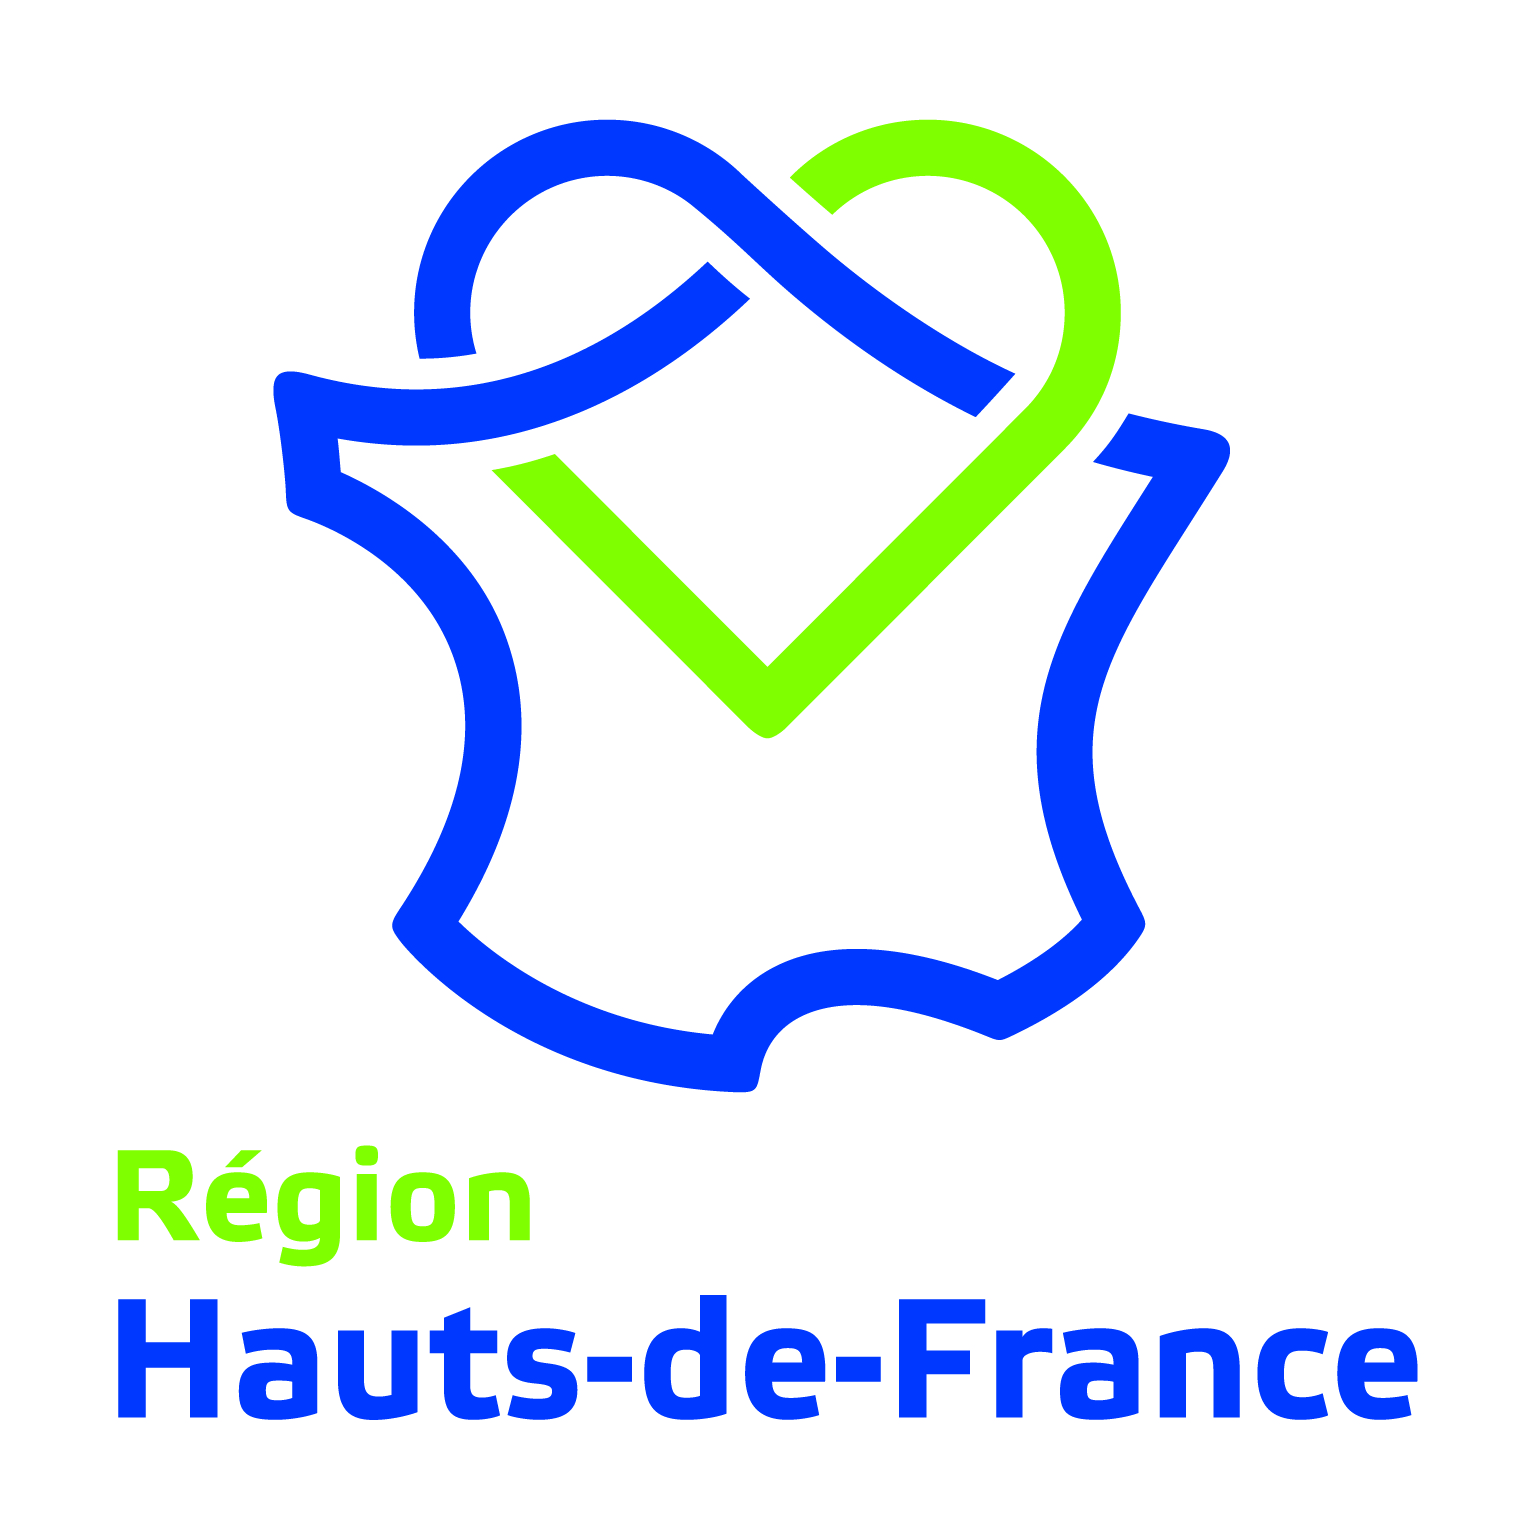
\includegraphics[width=\linewidth]{src/Figures/Introduction/Logo_HdF.jpg} 
    \caption*{}
    \label{fig-introduction:logo-hdf}
\end{wrapfigure}

    % Introduction
This doctoral research was conducted at Gustave Eiffel University\footnote{
    Gustave Eiffel University is an \acrfull{EPSCP}, founded in 2020 \textcolor{blue}{\autocite{universite_gustave_eiffel_notre_2024}}\index{Université Gustave Eiffel@\textsl{Université Gustave Eiffel}|pagebf}. It resulted from the merger and consolidation of a university, a research organization, and several schools, including notably \acrfull{IFSTTAR}, \acrfull{UPEM}, and other associated institutions.
}, within the \acrfull{LVMT}\footnote{
    The \acrfull{LVMT} is a \acrfull{UMR} founded in 2003, under the joint supervision of Gustave Eiffel University and the Institut Polytechnique de Paris, the latter being formed from a merger that notably included \acrfull{ENPC}. The \acrshort{LVMT} focuses on the study of the interactions between territories, transport, and mobility, utilizing multidisciplinary approaches from urban planning, geography, economics, sociology, anthropology, and engineering sciences \textcolor{blue}{\autocite{laboratoire_ville_mobilite_transport_presentation_2024}}\index{Laboratoire Ville Mobilité Transport@\textsl{Laboratoire Ville Mobilité Transport}|pagebf}.
}. The doctoral contract was co-financed by the Hauts-de-France Region, within the framework of the \textsl{rev3} initiative (\textsl{Third Industrial Revolution})\footnote{
    The \textsl{rev3} initiative (\textsl{Third Industrial Revolution}) is a collective dynamic launched in 2013, co-led by the Hauts-de-France Region and the \acrfull{CCI} Hauts-de-France. It aims to design and promote innovative territorial development models, set within a sustainable perspective towards 2050 \textcolor{blue}{\autocite{rev3_rev3_2022}}\index{rev3@\textsl{rev3}|pagebf}.
}. This doctoral thesis aligns with the second \acrfull{COP} 2023-2025 of Gustave Eiffel University\footnote{
    It particularly aligns with Strategic Project~2.1 (\Commas{Developing decarbonized mobility for all users and across all territories safely, based on the understanding of mobility behaviors and usage}) and~2.4 (\Commas{Progressing in development models integrating the Sustainable Development Goals}).
} and with the third research axis \Commas{Urban Planning and Territories}\footnote{
    Axis~3 \Commas{Urban Planning and Territories} of the \acrfull{LVMT} focuses on the study of interactions between territories, transport, and mobility \textcolor{blue}{\autocite{laboratoire_ville_mobilite_transport_axe_2024}}\index{Laboratoire Ville Mobilité Transport@\textsl{Laboratoire Ville Mobilité Transport}|pagebf}. It explores territorial dynamics and their modeling, transport network connections, urban planning models, and energy efficiency challenges. Research in this field revolves around two main levels of interaction. On one hand, it examines transport hubs, analyzing the flows they polarize, the developments they generate, and their strategic role for public and private actors. On the other hand, it studies how transport networks contribute to strengthening the links between territories, while influencing urban forms and relationships within regional urban systems.
} of the \acrshort{LVMT}.%%Translated%%
